% Please do not change the document class
\documentclass{scrartcl}

% Please do not change these packages
\usepackage[hidelinks]{hyperref}
\usepackage[none]{hyphenat}
\usepackage{setspace}
\doublespace

% You may add additional packages here
\usepackage{amsmath}
\usepackage{graphicx} 
\graphicspath{ {Diagrams/} }

% Please include a clear, concise, and descriptive title
\title{ Companion AI using a Behaviour Tree }

% Please do not change the subtitle
\subtitle{COMP230 - Game Component}

% Please put your student number in the author field
\author{1507866}

\begin{document}
	
\maketitle
	
\section{Outline}
My component is companion animal AI. My prototype is based on a Falcon.


The base version is based on birds - fight or flight


\begin{figure}[h]
	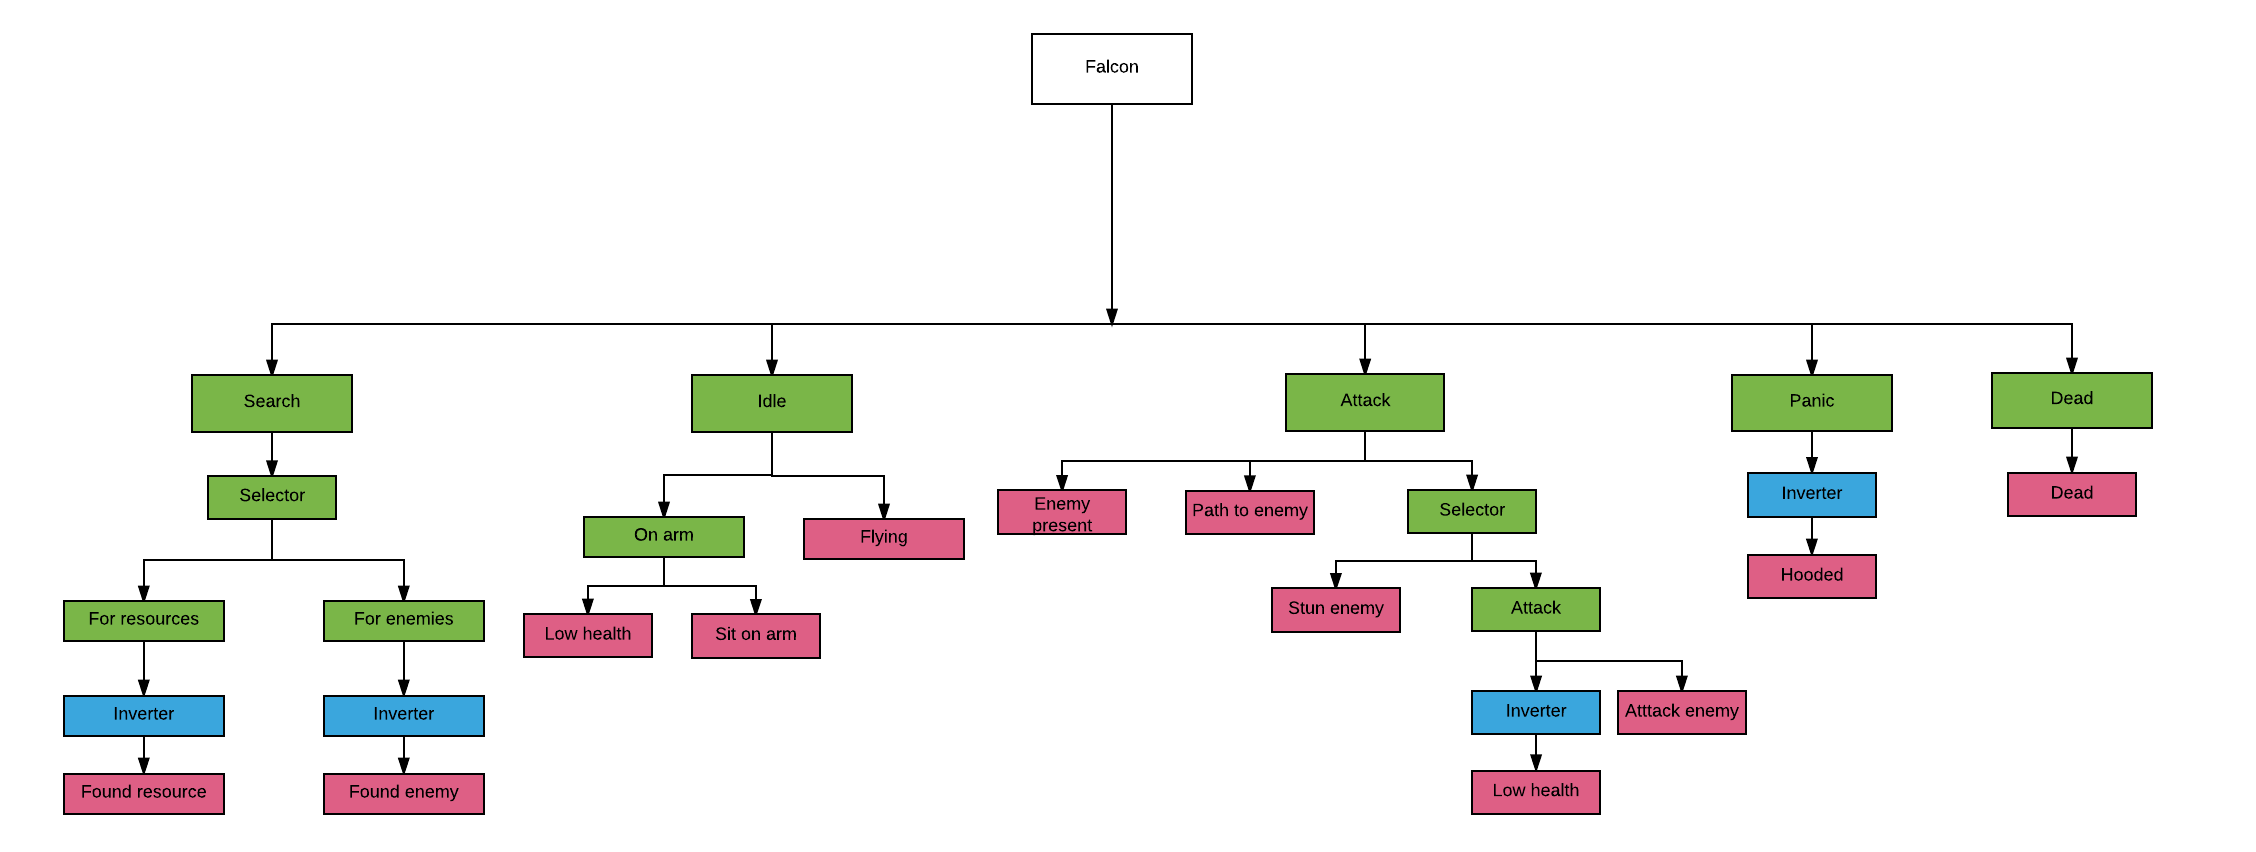
\includegraphics[width=1.2\linewidth]{behaviour_tree.png}
	\caption{ Behaviour tree being used on a falcon companion}
\end{figure} 


\section{Market Research}
Companion AI's tend to be people....

Games with dog AI like dragon age...

VR games using floaty robots...

Birds rarely used ... more environment / background

companion AI system 
should be easy to adapt to other animals

\bibliographystyle{ieeetr}
%\bibliography{comp230_1}
	
\end{document}
